\documentclass{standalone}

% Fontspec fot XeLaTeX
\usepackage{fontspec}
	% Unicode fonts
	\setmainfont{CMU Serif}

\usepackage{unicode-math}

\usepackage{tikz}
\usetikzlibrary{decorations.pathmorphing}

\newcommand{\rSch}{R_\text{S}} % Schwarzschild radius
\usepackage{amsmath}

\begin{document}
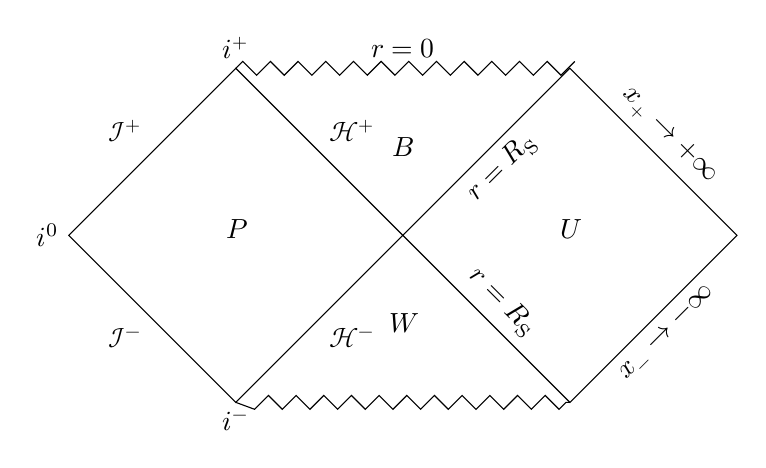
\begin{tikzpicture}%[scale=2]
\pgfmathsetmacro\myunit{3} 
	\draw (0,0)
			node [left] {$i^0$} 
		--++(45:\myunit)
			node [above]{$i^+$}
			coordinate (a)
			node [below = 1.8 cm] {$P$}
			node [pos = .5, above left] {$\mscrI^+$}
			% node [pos=.5, below, sloped] {$\bar{u}=\infty$}
		--++(-45:2*\myunit)
			node [pos = .25, above right] {$\mscrH^+$}
			node [pos = .75, above, sloped] {$r = \rSch$}%x_+ \to -\infty$}
			coordinate (d)	
			%node [below]{$i^-$}
		--++(45:\myunit)
			node [pos = .5, below, sloped] {$x_- \to -\infty$}
			% node [right] {$i^0$}
		--++(135:\myunit)
			% node [above] {$i^+$}
			node [below = 1.8 cm] {$U$}
			coordinate (b)
			node [pos = .5, above, sloped] {$x_+ \to +\infty$}
		--++(-135:2*\myunit)
			coordinate (c)
			node [pos = .25, below, sloped] {$r = \rSch$}%x_- \to +\infty$}
			node [pos = .75, below right] {$\mscrH^-$}
			node [below] {$i^-$}
		--cycle
			node [pos = .5, below left] {$\mscrI^-$};

 \draw [decorate, decoration=zigzag] (a) -- node [above] {$r=0$} % =6pt
											node [below = .75 cm] {$B$}
											(b) 

									 (c) -- node [above = .75 cm] {$W$}
											(d);

\end{tikzpicture}
\end{document}